\documentclass{beamer}
% Blocks, columns, a graphic, a table and a footnote inside frames.
% figure.png is tests/grok-corpus/images/clean-quadratic-formula.png
% (469 x 286 px), copied so the fixture is self-contained.
\usepackage{graphicx}
\usepackage{booktabs}
\setbeamertemplate{navigation symbols}{}

\title{Blocks and Columns}
\author{S. Liang}
\date{March 2026}

\begin{document}

\begin{frame}
  \titlepage
\end{frame}

\begin{frame}
  \frametitle{Three kinds of block}
  \begin{block}{Definition}
    A frame is the unit of a presentation; a slide is one overlay of a frame.
  \end{block}
  \begin{alertblock}{Caution}
    The frame counter and the page counter differ as soon as a frame has
    more than one slide.
  \end{alertblock}
  \begin{exampleblock}{Example}
    A frame with two \texttt{\textbackslash pause} commands has three slides.
  \end{exampleblock}
\end{frame}

\begin{frame}
  \frametitle{Two columns}
  \begin{columns}[T]
    \column{.5\textwidth}
      Left column, aligned at the top. This text is long enough to wrap
      inside its column so that the column width can be measured.
      \begin{itemize}
        \item first point
        \item second point
      \end{itemize}
    \column{.5\textwidth}
      Right column, also top-aligned, with a block inside it.
      \begin{block}{In a column}
        Blocks take the width of the column that contains them.
      \end{block}
  \end{columns}
\end{frame}

\begin{frame}
  \frametitle{A graphic}
  \begin{center}
    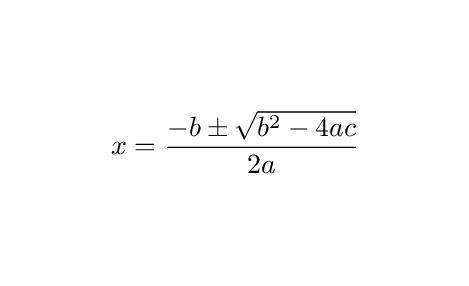
\includegraphics[width=.6\textwidth]{figure.png}
  \end{center}
  The image is scaled to six tenths of the text width and centred.
\end{frame}

\begin{frame}
  \frametitle{A table}
  \begin{table}
    \centering
    \begin{tabular}{lrr}
      \toprule
      stage & time (ms) & share \\
      \midrule
      parse   &  12 &  8\,\% \\
      shape   &  95 & 63\,\% \\
      break   &  31 & 21\,\% \\
      export  &  12 &  8\,\% \\
      \bottomrule
    \end{tabular}
    \caption{Time per stage for a ten-page document.}
  \end{table}
\end{frame}

\begin{frame}
  \frametitle{A footnote}
  Beamer puts footnotes at the bottom of the frame,\footnote{Above the
  footline, if the theme has one.} not at the bottom of the paper.

  \begin{block}{Blocks and columns together}
    \begin{columns}
      \column{.4\textwidth}
        narrow
      \column{.6\textwidth}
        wide, with more text than the narrow column so it wraps
    \end{columns}
  \end{block}
\end{frame}

\end{document}
